\documentclass[]{article}
\usepackage{lmodern}
\usepackage{amssymb,amsmath}
\usepackage{ifxetex,ifluatex}
\usepackage{fixltx2e} % provides \textsubscript
\ifnum 0\ifxetex 1\fi\ifluatex 1\fi=0 % if pdftex
  \usepackage[T1]{fontenc}
  \usepackage[utf8]{inputenc}
\else % if luatex or xelatex
  \ifxetex
    \usepackage{mathspec}
  \else
    \usepackage{fontspec}
  \fi
  \defaultfontfeatures{Ligatures=TeX,Scale=MatchLowercase}
\fi
% use upquote if available, for straight quotes in verbatim environments
\IfFileExists{upquote.sty}{\usepackage{upquote}}{}
% use microtype if available
\IfFileExists{microtype.sty}{%
\usepackage{microtype}
\UseMicrotypeSet[protrusion]{basicmath} % disable protrusion for tt fonts
}{}
\usepackage[margin=1in]{geometry}
\usepackage{hyperref}
\hypersetup{unicode=true,
            pdftitle={Record Linkage in Consumer Products Data using Approximate String Matching and Clustering Methods},
            pdfauthor={Riki Saito},
            pdfborder={0 0 0},
            breaklinks=true}
\urlstyle{same}  % don't use monospace font for urls
\usepackage{color}
\usepackage{fancyvrb}
\newcommand{\VerbBar}{|}
\newcommand{\VERB}{\Verb[commandchars=\\\{\}]}
\DefineVerbatimEnvironment{Highlighting}{Verbatim}{commandchars=\\\{\}}
% Add ',fontsize=\small' for more characters per line
\usepackage{framed}
\definecolor{shadecolor}{RGB}{248,248,248}
\newenvironment{Shaded}{\begin{snugshade}}{\end{snugshade}}
\newcommand{\KeywordTok}[1]{\textcolor[rgb]{0.13,0.29,0.53}{\textbf{{#1}}}}
\newcommand{\DataTypeTok}[1]{\textcolor[rgb]{0.13,0.29,0.53}{{#1}}}
\newcommand{\DecValTok}[1]{\textcolor[rgb]{0.00,0.00,0.81}{{#1}}}
\newcommand{\BaseNTok}[1]{\textcolor[rgb]{0.00,0.00,0.81}{{#1}}}
\newcommand{\FloatTok}[1]{\textcolor[rgb]{0.00,0.00,0.81}{{#1}}}
\newcommand{\ConstantTok}[1]{\textcolor[rgb]{0.00,0.00,0.00}{{#1}}}
\newcommand{\CharTok}[1]{\textcolor[rgb]{0.31,0.60,0.02}{{#1}}}
\newcommand{\SpecialCharTok}[1]{\textcolor[rgb]{0.00,0.00,0.00}{{#1}}}
\newcommand{\StringTok}[1]{\textcolor[rgb]{0.31,0.60,0.02}{{#1}}}
\newcommand{\VerbatimStringTok}[1]{\textcolor[rgb]{0.31,0.60,0.02}{{#1}}}
\newcommand{\SpecialStringTok}[1]{\textcolor[rgb]{0.31,0.60,0.02}{{#1}}}
\newcommand{\ImportTok}[1]{{#1}}
\newcommand{\CommentTok}[1]{\textcolor[rgb]{0.56,0.35,0.01}{\textit{{#1}}}}
\newcommand{\DocumentationTok}[1]{\textcolor[rgb]{0.56,0.35,0.01}{\textbf{\textit{{#1}}}}}
\newcommand{\AnnotationTok}[1]{\textcolor[rgb]{0.56,0.35,0.01}{\textbf{\textit{{#1}}}}}
\newcommand{\CommentVarTok}[1]{\textcolor[rgb]{0.56,0.35,0.01}{\textbf{\textit{{#1}}}}}
\newcommand{\OtherTok}[1]{\textcolor[rgb]{0.56,0.35,0.01}{{#1}}}
\newcommand{\FunctionTok}[1]{\textcolor[rgb]{0.00,0.00,0.00}{{#1}}}
\newcommand{\VariableTok}[1]{\textcolor[rgb]{0.00,0.00,0.00}{{#1}}}
\newcommand{\ControlFlowTok}[1]{\textcolor[rgb]{0.13,0.29,0.53}{\textbf{{#1}}}}
\newcommand{\OperatorTok}[1]{\textcolor[rgb]{0.81,0.36,0.00}{\textbf{{#1}}}}
\newcommand{\BuiltInTok}[1]{{#1}}
\newcommand{\ExtensionTok}[1]{{#1}}
\newcommand{\PreprocessorTok}[1]{\textcolor[rgb]{0.56,0.35,0.01}{\textit{{#1}}}}
\newcommand{\AttributeTok}[1]{\textcolor[rgb]{0.77,0.63,0.00}{{#1}}}
\newcommand{\RegionMarkerTok}[1]{{#1}}
\newcommand{\InformationTok}[1]{\textcolor[rgb]{0.56,0.35,0.01}{\textbf{\textit{{#1}}}}}
\newcommand{\WarningTok}[1]{\textcolor[rgb]{0.56,0.35,0.01}{\textbf{\textit{{#1}}}}}
\newcommand{\AlertTok}[1]{\textcolor[rgb]{0.94,0.16,0.16}{{#1}}}
\newcommand{\ErrorTok}[1]{\textcolor[rgb]{0.64,0.00,0.00}{\textbf{{#1}}}}
\newcommand{\NormalTok}[1]{{#1}}
\usepackage{longtable,booktabs}
\usepackage{graphicx,grffile}
\makeatletter
\def\maxwidth{\ifdim\Gin@nat@width>\linewidth\linewidth\else\Gin@nat@width\fi}
\def\maxheight{\ifdim\Gin@nat@height>\textheight\textheight\else\Gin@nat@height\fi}
\makeatother
% Scale images if necessary, so that they will not overflow the page
% margins by default, and it is still possible to overwrite the defaults
% using explicit options in \includegraphics[width, height, ...]{}
\setkeys{Gin}{width=\maxwidth,height=\maxheight,keepaspectratio}
\IfFileExists{parskip.sty}{%
\usepackage{parskip}
}{% else
\setlength{\parindent}{0pt}
\setlength{\parskip}{6pt plus 2pt minus 1pt}
}
\setlength{\emergencystretch}{3em}  % prevent overfull lines
\providecommand{\tightlist}{%
  \setlength{\itemsep}{0pt}\setlength{\parskip}{0pt}}
\setcounter{secnumdepth}{0}
% Redefines (sub)paragraphs to behave more like sections
\ifx\paragraph\undefined\else
\let\oldparagraph\paragraph
\renewcommand{\paragraph}[1]{\oldparagraph{#1}\mbox{}}
\fi
\ifx\subparagraph\undefined\else
\let\oldsubparagraph\subparagraph
\renewcommand{\subparagraph}[1]{\oldsubparagraph{#1}\mbox{}}
\fi

%%% Use protect on footnotes to avoid problems with footnotes in titles
\let\rmarkdownfootnote\footnote%
\def\footnote{\protect\rmarkdownfootnote}

%%% Change title format to be more compact
\usepackage{titling}

% Create subtitle command for use in maketitle
\newcommand{\subtitle}[1]{
  \posttitle{
    \begin{center}\large#1\end{center}
    }
}

\setlength{\droptitle}{-2em}
  \title{Record Linkage in Consumer Products Data using Approximate String
Matching and Clustering Methods}
  \pretitle{\vspace{\droptitle}\centering\huge}
  \posttitle{\par}
  \author{Riki Saito}
  \preauthor{\centering\large\emph}
  \postauthor{\par}
  \predate{\centering\large\emph}
  \postdate{\par}
  \date{November 23, 2016}

\begin{document}
\maketitle

\newpage

\tableofcontents
\newpage

\section{Preface}\label{preface}

This academic paper is submitted for the degree of Master of Science at
the University of Minnesota - Twin Cities. The study was conducted under
the supervision of Professor Xiaoou Li in the Department of Statistics,
University of Minnesota, during Fall of 2016.

XXX

\section{Background}\label{background}

We have all heard that we live in the age of data. Data is so accessible
and freely available, which has created a paradigm shift in how
analytics are done in many communities.

But the fact is, we have so much data that many of us do not know how to
use it or what to do with them. Data can be obtained in large quantities
and from multiple sources, which creates the struggle of cleaning the
data and making data usable.

This struggle is prevalent in many, if not all, of the business
industries. In this study we will focus on analytics in the
manufacturing industry, on dealing with data related to consumer
products.

Consumer product data (sales data), is an absolute necessity for any
business to do any sort of analytics. Sales data are generally available
by product and date-time, and analyses are conducted in various ways.
For example the sales performance of products can be evaluated for
specific dates or aggegated time periods (by month, season, year, etc).
Estimations of the percentage of shares the products dominate the market
can also be obtained and compared against the performance of competitor
products in the same market. These sort of analyses are essential in
business strategy and decision making.

Today, consumer product data is widely available and can be obtained
easily. Many businesses often use third party for-purchase data sources
from market research companies such as NPD or GFK. However, a large
issue in joining or aggregating data on consumer products is that,
compared to data like medical records of individuals, there are a lot
more ways of representing duplicate records, and the data
structure/hierarchy may not be clearly outlined. We define some key
terms for this paper:

\subsection{Definitions}\label{definitions}

\textbf{Product Line (PL)}: a group of products comprising of different
sizes, colors, or types, produced or sold under one unique product or
model name (i.e.~Apple iPhone 5, UE Boom 2)

\textbf{Stocking Keeping Unit (SKU)}: a particular product identified by
its product line as well as by its size, color, or type, where its
identification is typically used for inventory purposes (i.e.~Apple
iPhone 5 64GB Black, UE Boom 2 Blue)

\textbf{Distance}: an estimated numerical representation of how far
apart two objects are. Can be interchangeable with
\textbf{Dissimilarity}

\textbf{Group}: The actual class of one or more record(s) that belong to
the same entity

\textbf{Cluster}: The predicted class of one or more record(s) that
belong to the same entity

\textbf{Block}: A set or grouping of observations consisting of one or
more classes, grouped by higher-order variables (i.e.~list of SKU within
a Product Category and Brand)

\subsection{Record Linkage in Consumer Product
Data}\label{record-linkage-in-consumer-product-data}

Record linkage is a data cleaning task of identifying records that
belong to the same entity in a single data set or across multiple data
sets. An entity

It is necessary in aggregating or joining data by some entity that may
contain duplicates but do not share a common unique identifier due to
slight differences or inconsistencies. Compared to a ``brute force''
approach of linking records by hand, record linkage is an elegant
solution to combining duplicate, redundant, or even similar (but not
quite the same) records. It has applications in a wide variety of
fields; for instance, in health data linking medical records of the same
individuals may be necessary.

In this paper we focus on the application of record linkage in consumer
product data. A typical consumer products data hierarchy might appear
like this:

\begin{longtable}[]{@{}lll@{}}
\caption{Consumer Product Data Hierarchy}\tabularnewline
\toprule
\begin{minipage}[b]{0.18\columnwidth}\raggedright\strut
Data Hierarchy\strut
\end{minipage} & \begin{minipage}[b]{0.34\columnwidth}\raggedright\strut
Description\strut
\end{minipage} & \begin{minipage}[b]{0.38\columnwidth}\raggedright\strut
Example\strut
\end{minipage}\tabularnewline
\midrule
\endfirsthead
\toprule
\begin{minipage}[b]{0.18\columnwidth}\raggedright\strut
Data Hierarchy\strut
\end{minipage} & \begin{minipage}[b]{0.34\columnwidth}\raggedright\strut
Description\strut
\end{minipage} & \begin{minipage}[b]{0.38\columnwidth}\raggedright\strut
Example\strut
\end{minipage}\tabularnewline
\midrule
\endhead
\begin{minipage}[t]{0.18\columnwidth}\raggedright\strut
Category\strut
\end{minipage} & \begin{minipage}[t]{0.34\columnwidth}\raggedright\strut
Category, or type of product\strut
\end{minipage} & \begin{minipage}[t]{0.38\columnwidth}\raggedright\strut
Pointing Devices\strut
\end{minipage}\tabularnewline
\begin{minipage}[t]{0.18\columnwidth}\raggedright\strut
Brand\strut
\end{minipage} & \begin{minipage}[t]{0.34\columnwidth}\raggedright\strut
Name of Brand or Company\strut
\end{minipage} & \begin{minipage}[t]{0.38\columnwidth}\raggedright\strut
Logitech\strut
\end{minipage}\tabularnewline
\begin{minipage}[t]{0.18\columnwidth}\raggedright\strut
Product Line\strut
\end{minipage} & \begin{minipage}[t]{0.34\columnwidth}\raggedright\strut
Name of Product Model\strut
\end{minipage} & \begin{minipage}[t]{0.38\columnwidth}\raggedright\strut
M325 Wireless Optical Scroll Mouse\strut
\end{minipage}\tabularnewline
\begin{minipage}[t]{0.18\columnwidth}\raggedright\strut
Stock Keeping Unit\strut
\end{minipage} & \begin{minipage}[t]{0.34\columnwidth}\raggedright\strut
Product, defined by its model and features (color, size, type,
etc)\strut
\end{minipage} & \begin{minipage}[t]{0.38\columnwidth}\raggedright\strut
M325 Wireless Optical Scroll Mouse, Brick Red\strut
\end{minipage}\tabularnewline
\bottomrule
\end{longtable}

Product sales data will typically include information on many of these
hierarchy levels, but they can often be incomplete. For instancee, sales
may be reported at the SKU level, but information about the Product Line
may not be available. Here is an example of how the data might appear:

\begin{longtable}[]{@{}ll@{}}
\caption{Example: Sales Data}\tabularnewline
\toprule
Product Line & SKU\tabularnewline
\midrule
\endfirsthead
\toprule
Product Line & SKU\tabularnewline
\midrule
\endhead
- & Product A Bluetooth Mobile Speaker Black\tabularnewline
- & Product A Bluetooth Mobile Speaker Green\tabularnewline
- & Product A Bluetooth Mobile Speaker Gray\tabularnewline
- & Product B Bluetooth Mobile Speaker Black\tabularnewline
- & Product B Bluetooth Mobile Speaker Red\tabularnewline
- & Product C Tablet Case for iPad Black\tabularnewline
- & Product C Tablet Case for iPad Gray\tabularnewline
\bottomrule
\end{longtable}

With this data we are not able to perform any analytics at the Product
Line Level. The goal of record linkage is to identify SKUs that belong
to the same Product Line and transform the data as such:

\begin{longtable}[]{@{}ll@{}}
\caption{Example: Sales Data, Transformed}\tabularnewline
\toprule
Product Line & SKU\tabularnewline
\midrule
\endfirsthead
\toprule
Product Line & SKU\tabularnewline
\midrule
\endhead
Product A & Product A Bluetooth Mobile Speaker Black\tabularnewline
Product A & Product A Bluetooth Mobile Speaker Green\tabularnewline
Product A & Product A Bluetooth Mobile Speaker Gray\tabularnewline
Product B & Product B Bluetooth Mobile Speaker Black\tabularnewline
Product B & Product B Bluetooth Mobile Speaker Red\tabularnewline
Product C & Product B Tablet Case for iPad Black\tabularnewline
Product C & Product B Tablet Case for iPad Gray\tabularnewline
\bottomrule
\end{longtable}

\subsection{Study goals}\label{study-goals}

The goal of this paper is to discuss methods to identify the groups of
SKUs that belong to the same Product Line.

Record Linkage will be performed in two steps:

\begin{enumerate}
\def\labelenumi{\arabic{enumi})}
\item
  Calculating a dissimilarity matrix using
  \textbf{Approximate String Matching}
\item
  Grouping product names together using \textbf{Clustering}
\end{enumerate}

\subsection{Motivation}\label{motivation}

A foolproof way of insuring that all records get linked correctly is by
``brute force'' (i.e.~manually linking records). Especially in data
where a mis-linkage is costly in the sense that it could potentially
pose a serious problem (for example, misidentifying two different
patients as the same person), there may be a need for some manual
linkage or manual inspection of record linkage. However a ``brute
force'' is also very costly in terms of time and labor, and is not
scalable. In scenarios with a large number of records, it is not
feasible.

Let's say we have n products and we compare every product to every other
product. Then we will have a total of \(\frac{(n^2 - n)}{2}\)
comparisons. Thus the number of comparisons quickly increases with n and
there a ``brute force'' is not scalable.

\section{Data}\label{data}

For this study we will use product listings from Amazon.com. The data is
obtained from listings related to electronics and eletronic accessories.
Raw data obtained is about 280 different listings.

We then simulated data from the raw data by making assumptions about the
construction of product names and distributions of product name
components.

\subsection{Raw Data}\label{raw-data}

We obtained data from the following categories (and their frequencies):

\begin{verbatim}
## 
##  Mobile Speakers Pointing Devices  Smartphone Case  Tablet Keyboard 
##              108               27               85               62
\end{verbatim}

Here is the frequency of the data by brand level:

\begin{verbatim}
## 
##        Amazon          Bose     Caseology           JBL      Logitech 
##            22            15            45            43            62 
##     Microsoft         NuVur      SHIELDON Ultimate Ears          ZAGG 
##             8            34             6            14            33
\end{verbatim}

Here is a preview of the raw data:

\begin{verbatim}
##          Category Brand                                        SKU Class
## 1 Mobile Speakers   JBL  JBL Clip Portable Bluetooth Speaker Black     7
## 2 Mobile Speakers   JBL   JBL Clip Portable Bluetooth Speaker Blue     7
## 3 Mobile Speakers   JBL   JBL Clip Portable Bluetooth Speaker Grey     7
## 4 Mobile Speakers   JBL JBL Clip Portable Bluetooth Speaker Purple     7
## 5 Mobile Speakers   JBL    JBL Clip Portable Bluetooth Speaker Red     7
\end{verbatim}

\subsection{Data Simulation}\label{data-simulation}

Using raw data and general assumptions made on the data, a simulation
scheme was created to generate large samples of data. In order to
develop a simulation scheme, we first defined the framework of the data.

In our data, \textbf{Category} and \textbf{Brand} are two levels of the
data hierarchy for which we have information. Record linkage is
performed for each Category-Brand groups. Therefore we need a simulation
scheme that generates random SKU names within a defined Category-Brand.
Thus we can ignore those two levels.

Therefore we need a simulation scheme that generates a list (or
\textbf{Block}) of SKUs and its class. In a given block there will be a
random number of classes, each of some random size, where the individual
observations are SKU names. Each of these SKU names will consist of a
random number of words, and the names are constructed randomly.

In general, the SKU names are constructed with words that are either
specific to the Product Line (e.g.~model name, type of product) or words
that are specific to the SKU (color, size, etc).

These are the mentioend components of the data values that we need to
randomly generate:

\begin{enumerate}
\def\labelenumi{\arabic{enumi}.}
\tightlist
\item
  \textbf{Number of Classes (Product Lines)}: In a given group, the
  number of classes vary. We will use a discrete uniform distribution
  using the range of the number of classes in the raw data (min = 2, max
  = 8).
\item
  \textbf{Size of class}: For each of the classes generated in
  \textbf{1.}, the number of SKUs in the class also varies (see Figure 5
  in Appendix). We roughly estimated this distribution using a Gamma
  distribution.
\item
  \textbf{Length of SKU}: After class size is determine, we generate SKU
  names. Since not all SKU names have the same number of words, we
  generate the SKU length randomly (see Figure 6 in Appendix). We
  roughly estimated this distribution using a Gamma distribution.
\item
  \textbf{Word type}: When generating a SKU name, words are sampled from
  a list of words produced from the original data. These words are
  separated into two lists: 1) Words that describe the product (Desc),
  and 2) Words that describe features of the SKU (SKU); e.g.~colors,
  size, etc. USing the raw data, a binomial probability of word type was
  computed by location in the entire description (see Figure 7 in
  Appendix). We roughly estimated this distribution using an exponential
  function.
\end{enumerate}

The data components are broken down as the following:

\begin{longtable}[]{@{}ll@{}}
\caption{Simulation Scheme}\tabularnewline
\toprule
\begin{minipage}[b]{0.47\columnwidth}\raggedright\strut
Component\strut
\end{minipage} & \begin{minipage}[b]{0.48\columnwidth}\raggedright\strut
Distribution\strut
\end{minipage}\tabularnewline
\midrule
\endfirsthead
\toprule
\begin{minipage}[b]{0.47\columnwidth}\raggedright\strut
Component\strut
\end{minipage} & \begin{minipage}[b]{0.48\columnwidth}\raggedright\strut
Distribution\strut
\end{minipage}\tabularnewline
\midrule
\endhead
\begin{minipage}[t]{0.47\columnwidth}\raggedright\strut
\# Classes (Product Lines)\strut
\end{minipage} & \begin{minipage}[t]{0.48\columnwidth}\raggedright\strut
\(\sim Uniform(2, 8)\)\strut
\end{minipage}\tabularnewline
\begin{minipage}[t]{0.47\columnwidth}\raggedright\strut
Class Size (\# SKUs in Class)\strut
\end{minipage} & \begin{minipage}[t]{0.48\columnwidth}\raggedright\strut
\(\sim \Gamma(k = 2.92, \theta = 0.61)\)\strut
\end{minipage}\tabularnewline
\begin{minipage}[t]{0.47\columnwidth}\raggedright\strut
Length of Description (\# Words in SKU)\strut
\end{minipage} & \begin{minipage}[t]{0.48\columnwidth}\raggedright\strut
\(\sim \Gamma(k = 4.07, \theta = 0.32)\)\strut
\end{minipage}\tabularnewline
\begin{minipage}[t]{0.47\columnwidth}\raggedright\strut
Word Type (Product vs.~SKU-descriptive)\strut
\end{minipage} & \begin{minipage}[t]{0.48\columnwidth}\raggedright\strut
P(Type = Product \textbar{} X) = \(1 - exp(-7.5(1-x))\)\strut
\end{minipage}\tabularnewline
\bottomrule
\end{longtable}

This is an example of what the simulated data looks like:

\begin{verbatim}
##                                                        SKU Class
## 1    pattern port parallax smartphone 984000297 crimson...     1
## 2            pattern port parallax smartphone dark into...     1
## 3  pattern port parallax smartphone minigreen 984000294...     1
## 4    pattern port parallax smartphone spontaneous light...     1
## 5                            dual fits clip micro matte...     2
## 6                      dual fits clip micro genbabyblue...     2
## 7                       dual fits clip micro purplepink...     2
## 8                              dual fits clip micro the...     2
## 9                    dual fits clip micro lteblackgreen...     2
## 10                        dual fits clip micro electric...     2
\end{verbatim}

\section{Methods}\label{methods}

In order to accomplish our goal of identifing SKUs that belong to the
same Product Line, we propose two steps. The first step is calculating a
distance or dissimilarity matrix, using Approximate String Matching. The
second step is calculating clusters of the SKUs using Clustering
methods. We will then use several evaluation measures to compare
performance.

The procedure is outline in Figure 1. From a list of SKUs, a
dissimilarty matrix is obtained, and then a clustering method is applied
on the matrix to obtain cluster. It is then evaluated with several
methods. (Note that in Figure 1, Weighted Optimal String Alignment and
Single-Link Hierarchical Clustering is used).

\begin{figure}
\centering
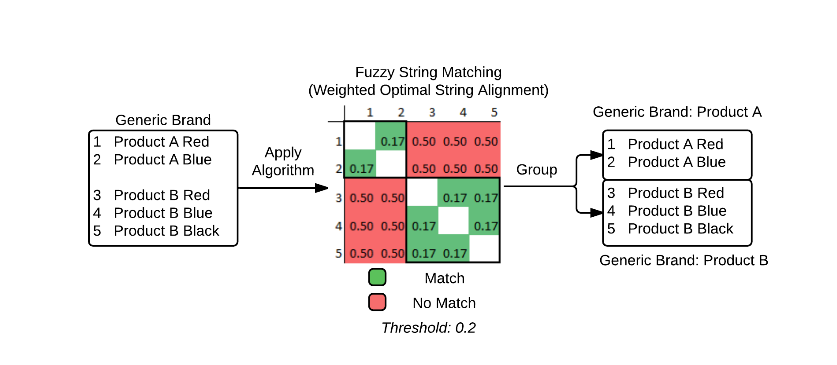
\includegraphics[width=300pt]{C:/Users/rjsai/Dropbox/UMN Courses/Plan B/wosa_process_bg.png}
\caption{Record Linkage Procedure}
\end{figure}

In our study our study we will apply and evalaute record linkage methods
on both the raw data and simulated data.

\subsection{Step 1: Approximate String
Matching}\label{step-1-approximate-string-matching}

Let's say for a given Product Category and Brand, we have a list of SKUs
similar to Table 2. Our end goal is to produce something like Table 3,
where we are able to accurately identify the correct group of Product
Lines. Let us consider these list of SKUs within a Product Category and
Brand as a \textbf{Block}.

Essentially what we are hoping to accomplish is match and group strings
that are very similar but not quite exactly the same. Some simple and
intuitive solutions would be to generate a substring of one string to
match another, or identify and remove irrelevant words, but these
solutions may not be the best solution simply because of the varied
structures of how these strings are constructed and the ambiguity in
determine whether words are irrelevant or not in identifying the product
line.

Approximate String Matching (also known as Fuzzy String Matching) is a
pattern matching algorithm that computes the degree of similartity
between two strings, and produces a quantitative metric of distance that
can be used to classify the strings as a match or not a match.

In this study, we will consider two algorithms:

\begin{longtable}[]{@{}ll@{}}
\caption{Approximate String Matching Algorithms
Considered}\tabularnewline
\toprule
\begin{minipage}[b]{0.32\columnwidth}\raggedright\strut
Method\strut
\end{minipage} & \begin{minipage}[b]{0.62\columnwidth}\raggedright\strut
Description\strut
\end{minipage}\tabularnewline
\midrule
\endfirsthead
\toprule
\begin{minipage}[b]{0.32\columnwidth}\raggedright\strut
Method\strut
\end{minipage} & \begin{minipage}[b]{0.62\columnwidth}\raggedright\strut
Description\strut
\end{minipage}\tabularnewline
\midrule
\endhead
\begin{minipage}[t]{0.32\columnwidth}\raggedright\strut
Optimal String Alignment (OSA)\strut
\end{minipage} & \begin{minipage}[t]{0.62\columnwidth}\raggedright\strut
calculates the ``edit distance'' between two strings\strut
\end{minipage}\tabularnewline
\begin{minipage}[t]{0.32\columnwidth}\raggedright\strut
Weighted Optimal String Alignment (WOSA)\strut
\end{minipage} & \begin{minipage}[t]{0.62\columnwidth}\raggedright\strut
calculates the ``edit distance'' between two strings, where edits are
weighted by location and determined by a function\strut
\end{minipage}\tabularnewline
\bottomrule
\end{longtable}

The Optimal String Alignment approach and the Weighted Optimal String
Alignment approach are different in its assumption about the data and
the computation of the distance.

\subsubsection{Optimal String Alignment}\label{optimal-string-alignment}

We will first discuss a classical approach called Optimal String
Alignemt (also known as Damerau Levenshtein Algorithm). It is an
algorithm that calculates the ``edit distance'' between two strings
\cite{Leven1966}. An ``edit'' is identified by one of these four:

\begin{longtable}[]{@{}lll@{}}
\caption{Edit Distance Operations (Levenshtein, 1966)}\tabularnewline
\toprule
Edit & Description & Example\tabularnewline
\midrule
\endfirsthead
\toprule
Edit & Description & Example\tabularnewline
\midrule
\endhead
Deletion & deletion of a single symbol & \textbf{b}eat -\textgreater{}
eat\tabularnewline
Insertion & insertion of a single symbol & eat -\textgreater{}
\textbf{b}eat\tabularnewline
Substitution & substitution of a single symbol with another &
\textbf{b}eat -\textgreater{} \textbf{h}eat\tabularnewline
Transposition & swapping of two adjacent symbols & be\textbf{at}
-\textgreater{} be\textbf{ta}\tabularnewline
\bottomrule
\end{longtable}

We will use the package \texttt{stringdist} in R to compute the edit
distance of the example from Table 2.

\begin{Shaded}
\begin{Highlighting}[]
\KeywordTok{library}\NormalTok{(stringdist)}
\NormalTok{a =}\StringTok{ "Product A Bluetooth Mobile Speaker Black"}
\NormalTok{b =}\StringTok{ "Product A Bluetooth Mobile Speaker Green"}
\KeywordTok{stringdist}\NormalTok{(a, b, }\DataTypeTok{method =} \StringTok{"osa"}\NormalTok{)}
\end{Highlighting}
\end{Shaded}

\begin{verbatim}
## [1] 5
\end{verbatim}

The edit distance is the number of edits required to transform one
description to the other, which is a total of 5 edits (\texttt{Black}
-\textgreater{} \texttt{Green}).

Let i = 1,\ldots{}, n be all the potential edit locations, \(x_{i}\) be
a binomial variable where 1 indicates edit at that location and 0
indicates no edit. Then edit distance can be converted into a score by
dividing by maximum number of possible edits (length of longer string).

\[
Score_{osa} = \frac{\sum_{i=1}^{n} x_{i}}{n}
\]

\begin{Shaded}
\begin{Highlighting}[]
\NormalTok{(}\DataTypeTok{n =} \KeywordTok{max}\NormalTok{(}\KeywordTok{nchar}\NormalTok{(a), }\KeywordTok{nchar}\NormalTok{(b)))}
\end{Highlighting}
\end{Shaded}

\begin{verbatim}
## [1] 40
\end{verbatim}

\begin{Shaded}
\begin{Highlighting}[]
\NormalTok{x.sum =}\StringTok{ }\KeywordTok{stringdist}\NormalTok{(a, b, }\DataTypeTok{method =} \StringTok{"osa"}\NormalTok{)}
\NormalTok{(}\DataTypeTok{score =} \NormalTok{x.sum/n)}
\end{Highlighting}
\end{Shaded}

\begin{verbatim}
## [1] 0.125
\end{verbatim}

With an edit distance of 5 and maximum number of edits of 40, the score
is 5/40, or 0.125, out of a maximum of 1.

The computation of distance using approximate string matching is quick
and scalable, and can have a very good performance with the right
selection of algorithm and parameters. However each algorithm has pros
and cons, and the appropriate selection of algorithm and parameters is
essential.

Optimal String Alignment is a fairly common algorithm used in practice
and has a wide range of application (XXX SOURCE). However, Optimal
String Alignment may not be the most appropriate algorithm in our case.

You may have noticed that the difference in model name is only one
``edit'', whereas the difference in SKU variation accounts for 11 single
edits. Out of the total number of edits possible (50 single-character
edits), we have a score of .24 out of a total score of 1, but only .02
of this is accounted by different product line, and the rest of the .22
are captured by the difference in SKU-specifc words. If our goal is to
identify matching product lines and not SKU, this method does not quite
satisfy our goal.

Here is an example scenario where this poses an issue

\begin{Shaded}
\begin{Highlighting}[]
\NormalTok{a =}\StringTok{ "Product A Bluetooth Mobile Speaker Black"}
\NormalTok{c =}\StringTok{ "Product B Bluetooth Mobile Speaker Black"}
\NormalTok{n =}\StringTok{ }\KeywordTok{max}\NormalTok{(}\KeywordTok{nchar}\NormalTok{(a), }\KeywordTok{nchar}\NormalTok{(c))}
\NormalTok{x.sum =}\StringTok{ }\KeywordTok{stringdist}\NormalTok{(a, c, }\DataTypeTok{method =} \StringTok{"osa"}\NormalTok{)}
\NormalTok{(}\DataTypeTok{score =} \NormalTok{x.sum/n)}
\end{Highlighting}
\end{Shaded}

\begin{verbatim}
## [1] 0.025
\end{verbatim}

We can see that even though SKU b and c belong to the same Product Line,
we end up with a closer distance between a and c with this method. Thus
Optimal String Alignment may not be appropriate, or need to be adjusted.
We need a method that is robust to differences in product line, not in
SKU.

\subsubsection{Weighted Optimal String
Alignment}\label{weighted-optimal-string-alignment}

The problem attributed to the Optimal String Alignment algorithm is that
differences in the two strings are weighted equally regardless of
location. We know that in these SKU descriptions, model names appear
towards the beginning of the string (the differences we WANT to
capture), while differences such as color variations or size appear
towards the end of the string (the difference we do not care about) (see
Figure 2). To summarise, we have these two general assumptions about the
SKU names :

\begin{enumerate}
\def\labelenumi{\arabic{enumi})}
\tightlist
\item
  Words specific to the SKU towards end of description
\item
  Words specific to the Product Line towards beginning of description
\end{enumerate}

\begin{figure}
\centering
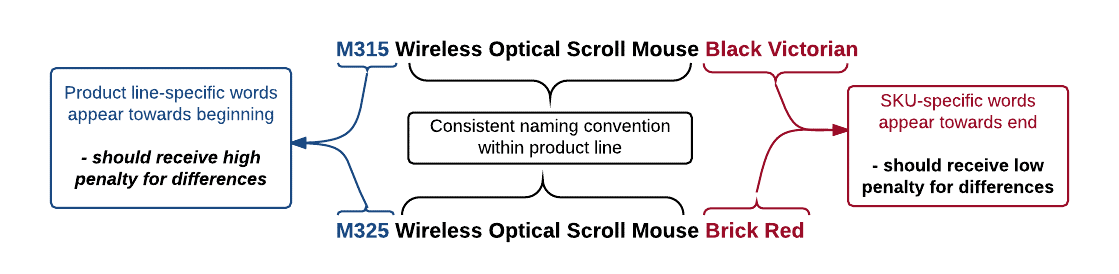
\includegraphics[width=300pt]{C:/Users/rjsai/Dropbox/UMN Courses/Plan B/phase1_assumptions.png}
\caption{Data Assumptions}
\end{figure}

Thus we introduce weights into the optimal string alignment, and call it
Weighted Optimal String Alignment. Weighted Optimal String Alignment is
currently not in existence in literature, but one that has potentailly
useful applications.

In Optimal string alignment, only the count of edits are considered.
However in Weighted Optimal String Alignment we consider the edits with
some weights determined by location.

Let i = 1,\ldots{}, n be all the potential edit locations, \(x_{i}\) be
a binomial variable where 1 indicates edit at that location and 0
indicates no edit, and \(w_{i}\) be the weight associated. Then,

\[
Score_{wosa} = \frac{\sum_{i=1}^{n} w_{i} x_{i}}{\sum_{1}^{n} w_{i}}
\]

For example, let us compare the classical optimal string alignment
approach to the weighted optimal string alignment approach. We consider
these two SKUs and determine the edit locations:

\begin{Shaded}
\begin{Highlighting}[]
\NormalTok{a =}\StringTok{ "Product A Bluetooth Mobile Speaker Black"}
\NormalTok{d =}\StringTok{ "Product B Bluetooth Mobile Speaker Red"}
\end{Highlighting}
\end{Shaded}

\begin{verbatim}
## [1]  9 36 37 38 39 40
\end{verbatim}

In the optimal string alignment approach we would simply take the count
of edits (6) divided by the total number of edits (n = 40), for a score
of 6/40.

However in Weighted Optimal String Alignment, we add weights to these
edits by location. Let us consider linear weights.

Then we create linear weights determined by length
\texttt{n\ =\ max(nchar(a),\ nchar(b))} and ranging from \texttt{n} to
\texttt{1}.

\begin{Shaded}
\begin{Highlighting}[]
\NormalTok{n =}\StringTok{ }\KeywordTok{max}\NormalTok{(}\KeywordTok{nchar}\NormalTok{(a), }\KeywordTok{nchar}\NormalTok{(c))}
\NormalTok{w =}\StringTok{ }\NormalTok{n:}\DecValTok{1}
\NormalTok{x =}\StringTok{ }\NormalTok{edits  }
\NormalTok{(}\DataTypeTok{score_osa =} \KeywordTok{sum}\NormalTok{(x)/n)}
\end{Highlighting}
\end{Shaded}

\begin{verbatim}
## [1] 0.15
\end{verbatim}

\begin{Shaded}
\begin{Highlighting}[]
\NormalTok{(}\DataTypeTok{score_wosa =} \KeywordTok{sum}\NormalTok{(w*x)/}\KeywordTok{sum}\NormalTok{(w))}
\end{Highlighting}
\end{Shaded}

\begin{verbatim}
## [1] 0.05731707
\end{verbatim}

Using this assumption about the data, we alter the algorithm by adding a
location-based weighting.

Here are other parameters are also considered in this algorithm.

\begin{longtable}[]{@{}lll@{}}
\caption{Parameters for Weighted Optimal String
Alignment}\tabularnewline
\toprule
\begin{minipage}[b]{0.15\columnwidth}\raggedright\strut
Parameter\strut
\end{minipage} & \begin{minipage}[b]{0.58\columnwidth}\raggedright\strut
Description\strut
\end{minipage} & \begin{minipage}[b]{0.15\columnwidth}\raggedright\strut
Default\strut
\end{minipage}\tabularnewline
\midrule
\endfirsthead
\toprule
\begin{minipage}[b]{0.15\columnwidth}\raggedright\strut
Parameter\strut
\end{minipage} & \begin{minipage}[b]{0.58\columnwidth}\raggedright\strut
Description\strut
\end{minipage} & \begin{minipage}[b]{0.15\columnwidth}\raggedright\strut
Default\strut
\end{minipage}\tabularnewline
\midrule
\endhead
\begin{minipage}[t]{0.15\columnwidth}\raggedright\strut
\texttt{type}\strut
\end{minipage} & \begin{minipage}[t]{0.58\columnwidth}\raggedright\strut
Option to apply algorithm by whole item or by single character. Since we
want to apply algorithm to WHOLE WORDS rather than single characters, by
item is ideal.\strut
\end{minipage} & \begin{minipage}[t]{0.15\columnwidth}\raggedright\strut
\texttt{character}\strut
\end{minipage}\tabularnewline
\begin{minipage}[t]{0.15\columnwidth}\raggedright\strut
\texttt{weight}\strut
\end{minipage} & \begin{minipage}[t]{0.58\columnwidth}\raggedright\strut
Weight function (linear, quadratic, root). In the previous example,
linear was used\strut
\end{minipage} & \begin{minipage}[t]{0.15\columnwidth}\raggedright\strut
\texttt{linear}\strut
\end{minipage}\tabularnewline
\begin{minipage}[t]{0.15\columnwidth}\raggedright\strut
\texttt{sum.right}\strut
\end{minipage} & \begin{minipage}[t]{0.58\columnwidth}\raggedright\strut
Flag for whether or not to consider everything after the first mismatch
(from the left-hand side) as mismatches (in other words, sum scores of
all mismatches to the right of first mismatch)\strut
\end{minipage} & \begin{minipage}[t]{0.15\columnwidth}\raggedright\strut
\texttt{F}\strut
\end{minipage}\tabularnewline
\bottomrule
\end{longtable}

(XXX Footnote add link to source code)

For our purpose, we will use \texttt{type\ =\ "item"} because this way
the length of the word (i.e.~number of characters) will not affect the
distance. We will also use \texttt{sum.right\ =\ T}, because we want to
identify difference in model (or Product Line) names, and any difference
occuring in the string after that should also be considered different.

For example we will take a look at how these two SKU names (that do not
belong to the same Product Line) will score under the default parameters
and the preferred paramters (for our scenario):

\begin{Shaded}
\begin{Highlighting}[]
\NormalTok{a =}\StringTok{ "Product A Bluetooth Mobile Speaker Black"}
\NormalTok{d =}\StringTok{ "Product B Bluetooth Mobile Speaker Red"}
\KeywordTok{wosa}\NormalTok{(a, d, }\DataTypeTok{type =} \StringTok{"character"}\NormalTok{, }\DataTypeTok{weight =} \StringTok{"linear"}\NormalTok{, }\DataTypeTok{sum.right =} \NormalTok{F)$score}
\end{Highlighting}
\end{Shaded}

\begin{verbatim}
## [1] 0.05731707
\end{verbatim}

\begin{Shaded}
\begin{Highlighting}[]
\KeywordTok{wosa}\NormalTok{(a, d, }\DataTypeTok{type =} \StringTok{"item"}\NormalTok{, }\DataTypeTok{weight =} \StringTok{"linear"}\NormalTok{, }\DataTypeTok{sum.right =} \NormalTok{T)$score}
\end{Highlighting}
\end{Shaded}

\begin{verbatim}
## [1] 0.7142857
\end{verbatim}

Under the preferred parameters we can see that the distance between the
two SKUs are large, and is therefore able to distinguish them well.

By applying OSA and WOSA to all pairs in a list of SKUs, we then obtain
distance matrices (Table 8 and 9).

\begin{longtable}[]{@{}ccllllll@{}}
\caption{Distance Matrix Optimal String Alignment}\tabularnewline
\toprule
\begin{minipage}[t]{0.36\columnwidth}\centering\strut
Product A Bluetooth Mobile Speaker Black\strut
\end{minipage} & \begin{minipage}[t]{0.05\columnwidth}\centering\strut
0\strut
\end{minipage} & \begin{minipage}[t]{0.05\columnwidth}\raggedright\strut
0.02\strut
\end{minipage} & \begin{minipage}[t]{0.05\columnwidth}\raggedright\strut
0.01\strut
\end{minipage} & \begin{minipage}[t]{0.05\columnwidth}\raggedright\strut
0.04\strut
\end{minipage} & \begin{minipage}[t]{0.05\columnwidth}\raggedright\strut
0.06\strut
\end{minipage} & \begin{minipage}[t]{0.05\columnwidth}\raggedright\strut
0.54\strut
\end{minipage} & \begin{minipage}[t]{0.05\columnwidth}\raggedright\strut
0.53\strut
\end{minipage}\tabularnewline
\begin{minipage}[t]{0.36\columnwidth}\centering\strut
Product A Bluetooth Mobile Speaker Green\strut
\end{minipage} & \begin{minipage}[t]{0.05\columnwidth}\centering\strut
0.02\strut
\end{minipage} & \begin{minipage}[t]{0.05\columnwidth}\raggedright\strut
0\strut
\end{minipage} & \begin{minipage}[t]{0.05\columnwidth}\raggedright\strut
0.01\strut
\end{minipage} & \begin{minipage}[t]{0.05\columnwidth}\raggedright\strut
0.06\strut
\end{minipage} & \begin{minipage}[t]{0.05\columnwidth}\raggedright\strut
0.05\strut
\end{minipage} & \begin{minipage}[t]{0.05\columnwidth}\raggedright\strut
0.54\strut
\end{minipage} & \begin{minipage}[t]{0.05\columnwidth}\raggedright\strut
0.53\strut
\end{minipage}\tabularnewline
\begin{minipage}[t]{0.36\columnwidth}\centering\strut
Product A Bluetooth Mobile Speaker Gray\strut
\end{minipage} & \begin{minipage}[t]{0.05\columnwidth}\centering\strut
0.01\strut
\end{minipage} & \begin{minipage}[t]{0.05\columnwidth}\raggedright\strut
0.01\strut
\end{minipage} & \begin{minipage}[t]{0.05\columnwidth}\raggedright\strut
0\strut
\end{minipage} & \begin{minipage}[t]{0.05\columnwidth}\raggedright\strut
0.05\strut
\end{minipage} & \begin{minipage}[t]{0.05\columnwidth}\raggedright\strut
0.05\strut
\end{minipage} & \begin{minipage}[t]{0.05\columnwidth}\raggedright\strut
0.53\strut
\end{minipage} & \begin{minipage}[t]{0.05\columnwidth}\raggedright\strut
0.53\strut
\end{minipage}\tabularnewline
\begin{minipage}[t]{0.36\columnwidth}\centering\strut
Product B Bluetooth Mobile Speaker Black\strut
\end{minipage} & \begin{minipage}[t]{0.05\columnwidth}\centering\strut
0.04\strut
\end{minipage} & \begin{minipage}[t]{0.05\columnwidth}\raggedright\strut
0.06\strut
\end{minipage} & \begin{minipage}[t]{0.05\columnwidth}\raggedright\strut
0.05\strut
\end{minipage} & \begin{minipage}[t]{0.05\columnwidth}\raggedright\strut
0\strut
\end{minipage} & \begin{minipage}[t]{0.05\columnwidth}\raggedright\strut
0.02\strut
\end{minipage} & \begin{minipage}[t]{0.05\columnwidth}\raggedright\strut
0.54\strut
\end{minipage} & \begin{minipage}[t]{0.05\columnwidth}\raggedright\strut
0.53\strut
\end{minipage}\tabularnewline
\begin{minipage}[t]{0.36\columnwidth}\centering\strut
Product B Bluetooth Mobile Speaker Red\strut
\end{minipage} & \begin{minipage}[t]{0.05\columnwidth}\centering\strut
0.06\strut
\end{minipage} & \begin{minipage}[t]{0.05\columnwidth}\raggedright\strut
0.05\strut
\end{minipage} & \begin{minipage}[t]{0.05\columnwidth}\raggedright\strut
0.05\strut
\end{minipage} & \begin{minipage}[t]{0.05\columnwidth}\raggedright\strut
0.02\strut
\end{minipage} & \begin{minipage}[t]{0.05\columnwidth}\raggedright\strut
0\strut
\end{minipage} & \begin{minipage}[t]{0.05\columnwidth}\raggedright\strut
0.53\strut
\end{minipage} & \begin{minipage}[t]{0.05\columnwidth}\raggedright\strut
0.53\strut
\end{minipage}\tabularnewline
\begin{minipage}[t]{0.36\columnwidth}\centering\strut
Product C Tablet Case for iPad Black\strut
\end{minipage} & \begin{minipage}[t]{0.05\columnwidth}\centering\strut
0.54\strut
\end{minipage} & \begin{minipage}[t]{0.05\columnwidth}\raggedright\strut
0.54\strut
\end{minipage} & \begin{minipage}[t]{0.05\columnwidth}\raggedright\strut
0.53\strut
\end{minipage} & \begin{minipage}[t]{0.05\columnwidth}\raggedright\strut
0.54\strut
\end{minipage} & \begin{minipage}[t]{0.05\columnwidth}\raggedright\strut
0.53\strut
\end{minipage} & \begin{minipage}[t]{0.05\columnwidth}\raggedright\strut
0\strut
\end{minipage} & \begin{minipage}[t]{0.05\columnwidth}\raggedright\strut
0.02\strut
\end{minipage}\tabularnewline
\begin{minipage}[t]{0.36\columnwidth}\centering\strut
Product C Tablet Case for iPad Gray\strut
\end{minipage} & \begin{minipage}[t]{0.05\columnwidth}\centering\strut
0.53\strut
\end{minipage} & \begin{minipage}[t]{0.05\columnwidth}\raggedright\strut
0.53\strut
\end{minipage} & \begin{minipage}[t]{0.05\columnwidth}\raggedright\strut
0.53\strut
\end{minipage} & \begin{minipage}[t]{0.05\columnwidth}\raggedright\strut
0.53\strut
\end{minipage} & \begin{minipage}[t]{0.05\columnwidth}\raggedright\strut
0.53\strut
\end{minipage} & \begin{minipage}[t]{0.05\columnwidth}\raggedright\strut
0.02\strut
\end{minipage} & \begin{minipage}[t]{0.05\columnwidth}\raggedright\strut
0\strut
\end{minipage}\tabularnewline
\bottomrule
\end{longtable}

\begin{longtable}[]{@{}ccllllll@{}}
\caption{Distance Matrix Weighted Optimal String
Alignment}\tabularnewline
\toprule
\begin{minipage}[t]{0.36\columnwidth}\centering\strut
Product A Bluetooth Mobile Speaker Black\strut
\end{minipage} & \begin{minipage}[t]{0.05\columnwidth}\centering\strut
0\strut
\end{minipage} & \begin{minipage}[t]{0.05\columnwidth}\raggedright\strut
0.05\strut
\end{minipage} & \begin{minipage}[t]{0.05\columnwidth}\raggedright\strut
0.05\strut
\end{minipage} & \begin{minipage}[t]{0.05\columnwidth}\raggedright\strut
0.71\strut
\end{minipage} & \begin{minipage}[t]{0.05\columnwidth}\raggedright\strut
0.71\strut
\end{minipage} & \begin{minipage}[t]{0.05\columnwidth}\raggedright\strut
0.75\strut
\end{minipage} & \begin{minipage}[t]{0.05\columnwidth}\raggedright\strut
0.75\strut
\end{minipage}\tabularnewline
\begin{minipage}[t]{0.36\columnwidth}\centering\strut
Product A Bluetooth Mobile Speaker Green\strut
\end{minipage} & \begin{minipage}[t]{0.05\columnwidth}\centering\strut
0.05\strut
\end{minipage} & \begin{minipage}[t]{0.05\columnwidth}\raggedright\strut
0\strut
\end{minipage} & \begin{minipage}[t]{0.05\columnwidth}\raggedright\strut
0.05\strut
\end{minipage} & \begin{minipage}[t]{0.05\columnwidth}\raggedright\strut
0.71\strut
\end{minipage} & \begin{minipage}[t]{0.05\columnwidth}\raggedright\strut
0.71\strut
\end{minipage} & \begin{minipage}[t]{0.05\columnwidth}\raggedright\strut
0.75\strut
\end{minipage} & \begin{minipage}[t]{0.05\columnwidth}\raggedright\strut
0.75\strut
\end{minipage}\tabularnewline
\begin{minipage}[t]{0.36\columnwidth}\centering\strut
Product A Bluetooth Mobile Speaker Gray\strut
\end{minipage} & \begin{minipage}[t]{0.05\columnwidth}\centering\strut
0.05\strut
\end{minipage} & \begin{minipage}[t]{0.05\columnwidth}\raggedright\strut
0.05\strut
\end{minipage} & \begin{minipage}[t]{0.05\columnwidth}\raggedright\strut
0\strut
\end{minipage} & \begin{minipage}[t]{0.05\columnwidth}\raggedright\strut
0.71\strut
\end{minipage} & \begin{minipage}[t]{0.05\columnwidth}\raggedright\strut
0.71\strut
\end{minipage} & \begin{minipage}[t]{0.05\columnwidth}\raggedright\strut
0.75\strut
\end{minipage} & \begin{minipage}[t]{0.05\columnwidth}\raggedright\strut
0.75\strut
\end{minipage}\tabularnewline
\begin{minipage}[t]{0.36\columnwidth}\centering\strut
Product B Bluetooth Mobile Speaker Black\strut
\end{minipage} & \begin{minipage}[t]{0.05\columnwidth}\centering\strut
0.71\strut
\end{minipage} & \begin{minipage}[t]{0.05\columnwidth}\raggedright\strut
0.71\strut
\end{minipage} & \begin{minipage}[t]{0.05\columnwidth}\raggedright\strut
0.71\strut
\end{minipage} & \begin{minipage}[t]{0.05\columnwidth}\raggedright\strut
0\strut
\end{minipage} & \begin{minipage}[t]{0.05\columnwidth}\raggedright\strut
0.05\strut
\end{minipage} & \begin{minipage}[t]{0.05\columnwidth}\raggedright\strut
0.75\strut
\end{minipage} & \begin{minipage}[t]{0.05\columnwidth}\raggedright\strut
0.75\strut
\end{minipage}\tabularnewline
\begin{minipage}[t]{0.36\columnwidth}\centering\strut
Product B Bluetooth Mobile Speaker Red\strut
\end{minipage} & \begin{minipage}[t]{0.05\columnwidth}\centering\strut
0.71\strut
\end{minipage} & \begin{minipage}[t]{0.05\columnwidth}\raggedright\strut
0.71\strut
\end{minipage} & \begin{minipage}[t]{0.05\columnwidth}\raggedright\strut
0.71\strut
\end{minipage} & \begin{minipage}[t]{0.05\columnwidth}\raggedright\strut
0.05\strut
\end{minipage} & \begin{minipage}[t]{0.05\columnwidth}\raggedright\strut
0\strut
\end{minipage} & \begin{minipage}[t]{0.05\columnwidth}\raggedright\strut
0.75\strut
\end{minipage} & \begin{minipage}[t]{0.05\columnwidth}\raggedright\strut
0.75\strut
\end{minipage}\tabularnewline
\begin{minipage}[t]{0.36\columnwidth}\centering\strut
Product C Tablet Case for iPad Black\strut
\end{minipage} & \begin{minipage}[t]{0.05\columnwidth}\centering\strut
0.75\strut
\end{minipage} & \begin{minipage}[t]{0.05\columnwidth}\raggedright\strut
0.75\strut
\end{minipage} & \begin{minipage}[t]{0.05\columnwidth}\raggedright\strut
0.75\strut
\end{minipage} & \begin{minipage}[t]{0.05\columnwidth}\raggedright\strut
0.75\strut
\end{minipage} & \begin{minipage}[t]{0.05\columnwidth}\raggedright\strut
0.75\strut
\end{minipage} & \begin{minipage}[t]{0.05\columnwidth}\raggedright\strut
0\strut
\end{minipage} & \begin{minipage}[t]{0.05\columnwidth}\raggedright\strut
0.04\strut
\end{minipage}\tabularnewline
\begin{minipage}[t]{0.36\columnwidth}\centering\strut
Product C Tablet Case for iPad Gray\strut
\end{minipage} & \begin{minipage}[t]{0.05\columnwidth}\centering\strut
0.75\strut
\end{minipage} & \begin{minipage}[t]{0.05\columnwidth}\raggedright\strut
0.75\strut
\end{minipage} & \begin{minipage}[t]{0.05\columnwidth}\raggedright\strut
0.75\strut
\end{minipage} & \begin{minipage}[t]{0.05\columnwidth}\raggedright\strut
0.75\strut
\end{minipage} & \begin{minipage}[t]{0.05\columnwidth}\raggedright\strut
0.75\strut
\end{minipage} & \begin{minipage}[t]{0.05\columnwidth}\raggedright\strut
0.04\strut
\end{minipage} & \begin{minipage}[t]{0.05\columnwidth}\raggedright\strut
0\strut
\end{minipage}\tabularnewline
\bottomrule
\end{longtable}

\subsection{Step 2: Unsupervised
Clustering}\label{step-2-unsupervised-clustering}

Using the distance/dissimilarity matrix for a block, we then using
clustering methods to predict the classes of the observations. Since in
reality we do not know the true classes (Product Line) of the
observations (SKUs), we need unsupervised methods. We do not even know
the number of clusters, so methods such as K-means would not be
appropriate. Here we will introduce the use of two clustering methods:
Hierarchica Clustering, and Density-Based Spectral Clustering (DBSCAN).

\subsubsection{Hierarchical Clustering}\label{hierarchical-clustering}

Hierarchical clustering, as the name implies, is a method that builds
clusters in a hierarchical manner. Hierarchies can be built in two ways.
In the Agglomerative approach, the hierarchy is built from the bottom up
where each observation starts in its own clusters, and is paired/grouped
as the observations are traced up on the hierarchy. The Divisive
approach works in the opposite manner, where we start with a single
large cluster of all observations, and observations are split
recursively from the top down and branching off into new clusters,
creating a hierarchy.

(XXX SOURCE
\url{http://nlp.stanford.edu/IR-book/html/htmledition/single-link-and-complete-link-clustering-1.html})

Hierarchical clustering has a variety of linkage criteria for
determining the distance between sets of observations. In our study we
will consider single-linkage and complete-linkage.

In the \textbf{single-linkage} clustering approach, the distance between
two clusters (or set of observations) is determined by the distance of
the closest members. This means that between two clusters we only
consider the points that have shortest distance possible. Thus the rest
of the cluster and the overall structure of the cluster is not taken
into consideration.

On the contrary, in the \textbf{complete-linkage} clustering approach,
the distance between two clusters (or set of observations) is determined
by the distance of the furthest members. In this approach, the overall
structure of the cluster is considered. One issue with this approach is
that the linkage will be sensitive to outliers, and single observations
within cluster that are further from the rest of the points can largely
affect the cluster's linkage with other clusters.

The arrangements of clusters in hierarchical clustering can be
visualized using Dendrogram, a type of tree diagram (see Figures 3 and
4). With the height (or distance) on the y-axis, the top of the tree
represents all observations under a single cluster, and from the top
down each node represents a split of the cluster into smaller clusters
at the corresponding height.

FIX single and complete will tell us about the structure of the clusters
and how that affects linkages

\begin{figure}
\centering
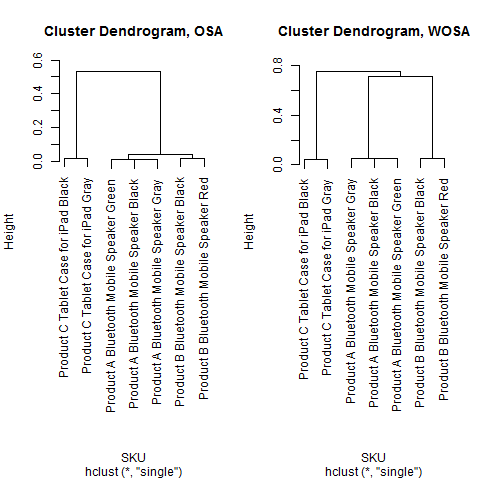
\includegraphics[width=280pt]{C:/Users/rjsai/Dropbox/UMN Courses/Plan B/figures/hc_single.png}
\caption{Dendrogram of Single-Link Hierarchical Clustering}
\end{figure}

\begin{figure}
\centering
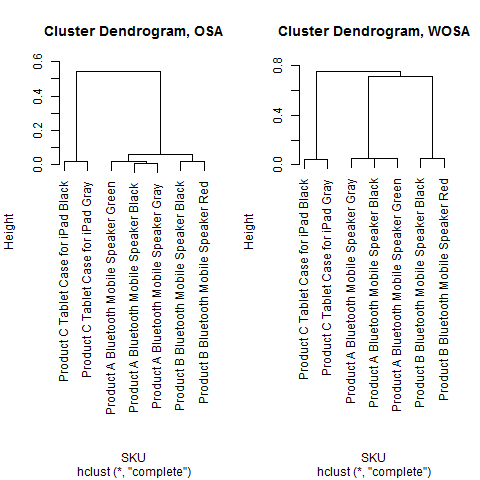
\includegraphics[width=280pt]{C:/Users/rjsai/Dropbox/UMN Courses/Plan B/figures/hc_complete.png}
\caption{Dendrogram of Complete-Link Hierarchical Clustering}
\end{figure}

There are two ways of obtaining clusters from hierarchical clustering;
one is to supply a number of clusters to obtain, and the other is to
supply a cutoff value to cut the dendrogram at. The former requires
prior knowledge on the number of clusters, and in our scenario we do not
have such information, so we proceed with the second way.

It is critical that an appropriate cutoff is selected: for example if a
cutoff is too high, then all the observations will be placed in one
cluster; if the cutoff is too low, every single observation will be in
its own cluster.

In Figures 3 we compare the OSA and WOSA distance matrices using
Single-link Hierarchical Clustering (and in Figure 4, Complete-link
Hierarchical Clustering).

A major flaw of the use of hierarchical clustering in our scenario is
the lack of an appropriate way of selecting the right cutoff value. In
general, hierarchical clustering is an exploratory method that allows
for visual exploration as in these dendrograms. Determine a cutoff value
is most commonly determined by inspecting the dendrogram and selecting
the cutoff where the vertical branches (uninterrupted by splits) is the
longest.

\subsubsection{Density-Based Spectral
Clustering}\label{density-based-spectral-clustering}

XXX FINISH

\url{https://en.wikipedia.org/wiki/DBSCAN}

``Consider a set of points in some space to be clustered. For the
purpose of DBSCAN clustering, the points are classified as core points,
(density-)reachable points and outliers, as follows: A point p is a core
point if at least minPts points are within distance \(\epsilon\) is the
maximum radius of the neighborhood from p) of it (including p). Those
points are said to be directly reachable from p.~By definition, no
points are directly reachable from a non-core point. A point q is
reachable from p if there is a path p1, \ldots{}, pn with p1 = p and pn
= q, where each pi+1 is directly reachable from pi (all the points on
the path must be core points, with the possible exception of q).

All points not reachable from any other point are outliers. Now if p is
a core point, then it forms a cluster together with all points (core or
non-core) that are reachable from it. Each cluster contains at least one
core point; non-core points can be part of a cluster, but they form its
``edge'', since they cannot be used to reach more points."

``A cluster then satisfies two properties: All points within the cluster
are mutually density-connected. If a point is density-reachable from any
point of the cluster, it is part of the cluster as well.''

\subsection{Evaluation}\label{evaluation}

There are several ways to compare the clusters to the actual class
(Product Line) of the observations (SKUs). Since not one evaluation
measure is better than the rest, we will consider a few of them
simultaneously.

The simplest of measures is the accuracy. In clustering, accuracy is
defined as:

\[
Accuracy = \frac{TP + TN}{P + N}
\]

Where P = all positives (number of within-cluster pairs), N = all
negative (number of between-cluster pairs), TP = true positives (number
of within-cluster pairs that are true), and NP = true negatives (number
of between-cluster pairs that are true).

Another measure that is commonly used in evaluating the performance of
clusters is known as purity, which is a measure of how ``pure'' each
cluster is. In the calculation of purity, for each cluster we count the
frequency of the most frequently-appearing class. That is then summed
and then divided by the total number of observations. Mathematically it
is defined as:

\[
Purity = \frac{1}{n}
  \sum_{q=1}^k \max_{1 \leq j \leq l} n_q^j ,
\]

where n is the total number of observations, q = 1,.., k is the cluster
index, j = i,..,. l is the class index, and \(n^{j}_{q}\) is the
frequency of class j in cluster q.

The problem with purity is that it is insensitive to the number of
clusters. Hypothetically, if every observation was in its own cluster,
then all clusters will have 100\% purity, and thus the total purity will
also be 100\%.

We will introduce one more measure, known as the \(F_{1}\) score (or
F-measure). The \(F_{1}\) score considers the harmonic mean of the
precision and recall, which are not considered in neither accuracy nor
purity. The \(F_{1}\) score is calculated as:

\[
F-score = \frac{2 \cdot Precision \cdot Recall}{Precision + Recall}
\]

where

\[
Precision = \frac{TP}{TP + FP} 
\]

and

\[
Recall = \frac{TP}{TP + FN} 
\]

FIX which evaluation measures to pay attention to

\section{Results}\label{results}

We will evaluate the results on two sets of data; one is the raw data
obtained from Amazon listings, and the other is simulated data. For the
simulated data we will also assess the run time of clustering methods.

We will evaluate the measures from the two Approximate String Alignment
algorithms (OSA and WOSA) and three clustering approaches
(single-link/complete-link Hierarchical Clustering, DBSCAN).

In general, WOSA will have a tendency to give a smaller score than OSA
for our kind of data, so for Hierarchical clustering, we have fixed the
cutoff value at 0.3 for OSA and 0.2 for WOSA. For the DBSCAN, we have
fixed the \(\epsilon\) value at 0.3 for DBSCAN.

\subsection{Simulation}\label{simulation}

\begin{longtable}[]{@{}llllll@{}}
\caption{Results (Simulation): Optimal String Alignment}\tabularnewline
\toprule
& Accuracy & Purity & Precision & Recall & F1 Score\tabularnewline
\midrule
\endfirsthead
\toprule
& Accuracy & Purity & Precision & Recall & F1 Score\tabularnewline
\midrule
\endhead
Hierarchical Clustering (Single-link) & 0.9092 & 1.0000 & 0.9600 &
0.6703 & 0.7475\tabularnewline
Hierarchical Clustering (Compete-link) & 0.9092 & 1.0000 & 0.9600 &
0.6703 & 0.7475\tabularnewline
DBSCAN & 0.9260 & 0.9081 & 0.8347 & 1.0000 & 0.8900\tabularnewline
\bottomrule
\end{longtable}

\begin{longtable}[]{@{}llllll@{}}
\caption{Results (Simulation): Weighed Optimal String
Alignment}\tabularnewline
\toprule
& Accuracy & Purity & Precision & Recall & F1 Score\tabularnewline
\midrule
\endfirsthead
\toprule
& Accuracy & Purity & Precision & Recall & F1 Score\tabularnewline
\midrule
\endhead
Hierarchical Clustering (Single-link) & 0.9531 & 1.0000 & 0.9900 &
0.8398 & 0.8835\tabularnewline
Hierarchical Clustering (Compete-link) & 0.9531 & 1.0000 & 0.9900 &
0.8398 & 0.8835\tabularnewline
DBSCAN & 0.9940 & 0.9946 & 0.9895 & 1.0000 & 0.9933\tabularnewline
\bottomrule
\end{longtable}

The simulation results tells us several things. One notable observation
is that the results from single-linkage vs.~complete-linkage
hierarchical clustering gives the same measures for all evaluations, and
presumptuously the same clustering results. This means that the
structure of clusters (as discussed in the Methods section) does not
have much influence on the cluster linkages. Another possible
explanation is that observations in each cluster is fairly compact
(close together), and separated well from other clusters.

The hierarchical clustering methods appear to give perfect purity and a
very high precision, but not so well in recall. This means that the
method is able to accurately separate observations that do not belong
together, but fails to identify a large number of observations that do
belong together. One cause of this could be from the cutoff value being
too conservative (too low). However, for OSA we are using a cutofff
value of 30\%, which in general is already on the larger side, so
perhaps the OSA algorithm is not appropriate.

On the other hand, DBSCAN has a good performance overall, especially
with WOSA. It is able to almost always accurately predict the correct
class, without sacrificing precision or recall.

\subsection{Raw Data}\label{raw-data-1}

The same Approximate String Matching and Clustering Methods were also
applied on the raw data. Here are the results.

\begin{longtable}[]{@{}llllll@{}}
\caption{Results (Raw Data): Optimal String Alignment}\tabularnewline
\toprule
& Accuracy & Purity & Precision & Recall & F1 Score\tabularnewline
\midrule
\endfirsthead
\toprule
& Accuracy & Purity & Precision & Recall & F1 Score\tabularnewline
\midrule
\endhead
Hierarchical Clustering (Single-link) & 0.9254 & 0.9470 & 0.8525 &
0.8301 & 0.8148\tabularnewline
Hierarchical Clustering (Compete-link) & 0.9254 & 0.9470 & 0.8525 &
0.8301 & 0.8148\tabularnewline
DBSCAN & 0.8663 & 0.8560 & 0.8283 & 0.9653 & 0.8454\tabularnewline
\bottomrule
\end{longtable}

\begin{longtable}[]{@{}llllll@{}}
\caption{Results (Raw Data): Weighed Optimal String
Alignment}\tabularnewline
\toprule
& Accuracy & Purity & Precision & Recall & F1 Score\tabularnewline
\midrule
\endfirsthead
\toprule
& Accuracy & Purity & Precision & Recall & F1 Score\tabularnewline
\midrule
\endhead
Hierarchical Clustering (Single-link) & 0.9277 & 0.9470 & 0.9359 &
0.8447 & 0.8243\tabularnewline
Hierarchical Clustering (Compete-link) & 0.9277 & 0.9470 & 0.9359 &
0.8447 & 0.8243\tabularnewline
DBSCAN & 0.9311 & 0.9135 & 0.8717 & 0.9721 & 0.8970\tabularnewline
\bottomrule
\end{longtable}

Again, we see that single-linkage and complete-linkage clustering gives
the same results. In general, the WOSA evaluation measures are better
than the OSA measures for hierarchical clustering.

DBSCAN does not always outperform Hierarchical Clustering, but the best
results from this whle table comes from DBSCAN with WOSA, with the
highest accuracy and F1 score measures, which is consistent with
simulation.

\section{Discussion}\label{discussion}

OSA vs.~WOSA Hierarchical Clustering vs.~DBSCAN

Results in Simulation vs.~Results in Raw Data

\section{Conclusion}\label{conclusion}

What went well/what can be improved

Extensions:

WOSA algorithm (or the idea of location weighting) can be applied to
other algorithms/problems

Application of WOSA to other data

Other clustering methods, tuning of parameters in clustering

\pagebreak

\section{Appendix}\label{appendix}

\begin{figure}
\centering
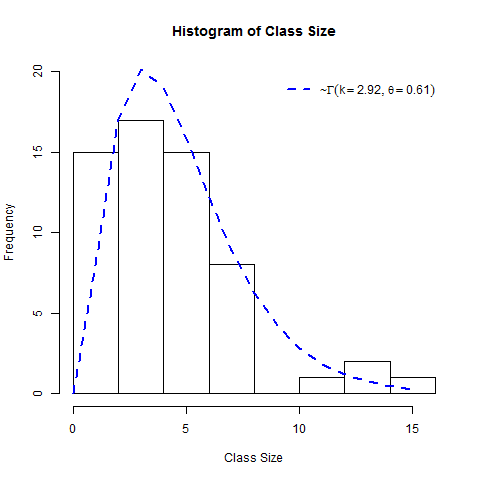
\includegraphics[width=280pt]{C:/Users/rjsai/Dropbox/UMN Courses/Plan B/figures/class_size_dist.png}
\caption{Dendrogram of Complete-Link Hierarchical Clustering}
\end{figure}

\begin{figure}
\centering
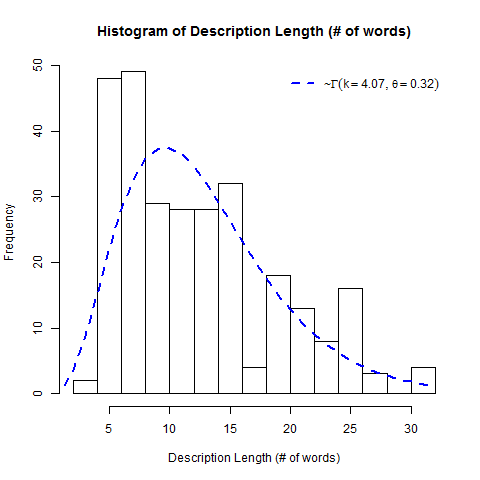
\includegraphics[width=280pt]{C:/Users/rjsai/Dropbox/UMN Courses/Plan B/figures/desc_length_dist.png}
\caption{Dendrogram of Complete-Link Hierarchical Clustering}
\end{figure}

\begin{figure}
\centering
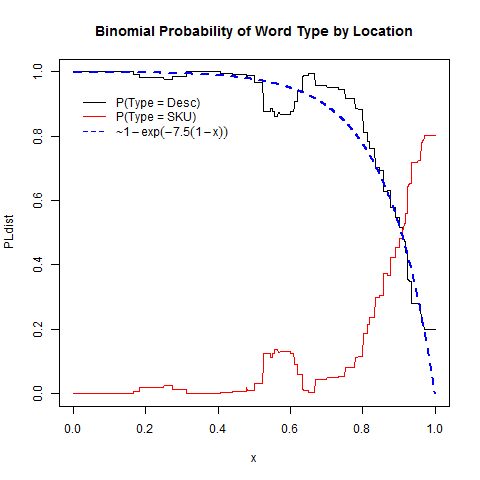
\includegraphics[width=280pt]{C:/Users/rjsai/Dropbox/UMN Courses/Plan B/figures/word_type_prob.png}
\caption{Dendrogram of Complete-Link Hierarchical Clustering}
\end{figure}

\newpage

\section{References}\label{references}

\renewcommand{\section}[2]{}%

\begin{thebibliography}{9}

\bibitem{Leven1966}
Vladimir I. Levenshtein, Binary codes capable of correcting deletions, insertions, and reversals, Doklady Akademii Nauk SSSR, 163(4):845-848, 1965 (Russian). English translation in Soviet Physics Doklady, 10(8):707-710, 1966.

\bibitem{Ariel2014} 
Ariel, A., Bakker, B. F. M., de Groot, M., van Grootheest, G., van der Laan, J., Smit, J., $\&$ Verkerk, B. (2014). Record Linkage in Health Data : a simulation study.

\bibitem{Christen2012}
Christen, P. (2012). A survey of indexing techniques for scalable record linkage and deduplication. IEEE Transactions on Knowledge and Data Engineering, 24(9), 1537-1555. \texttt{https://doi.org/10.1109/TKDE.2011.127}

\bibitem{Christen2007}
Christen, P., \& Goiser, K. (2007). Quality and complexity measures for data linkage and deduplication. Quality Measures in Data Mining, 151, 127-151. \texttt{https://doi.org/10.1007/978-3-540-44918-8\_6}

\bibitem{Zhao2002}
Zhao, Y., \& Karypis, G. (2002). Evaluation of Hierarchical Clustering Algorithms for Document Datasets, 515-524.

\bibitem{Gu2003}
Gu, L., \& Baxter, R. (2003). Record linkage: Current practice and future directions. Cmis, 03/83. Retrieved from \texttt{http://festivalofdoubt.uq.edu.au/papers/record\_linkage.pdf}

\bibitem{Winkler1983}
Winkler, W. E. (1983). MATCHING AND RECORD LINKAGE. U.S. Bureau of the Census. Evaluation.

\bibitem{Sauleau2005}
Sauleau, E. a, Paumier, J.-P., \& Buemi, A. (2005). Medical record linkage in health information systems by approximate string matching and clustering. BMC Medical Informatics and Decision Making, 5, 32. \texttt{https://doi.org/10.1186/1472-6947-5-32}

\bibitem{Ng2001}
Ng, A. Y., Jordan, M. I., \& Weiss, Y. (2001). On spectral clustering: Analysis and an algorithm. Advances in Neural Information Processing Systems 14, 849-856. \texttt{https://doi.org/10.1.1.19.8100}

\bibitem{VanderLoo2014}
van der Loo, M. (2014). {stringdist}: an {R} Package for Approximate String Matching. The R Journal, 6(1), 111-122.

\bibitem{Ester1996}
Ester, Martin, et al. "A density-based algorithm for discovering clusters in large spatial databases with noise." Kdd. Vol. 96. No. 34. 1996.

\end{thebibliography}


\end{document}
